\documentclass[11pt]{article}
\usepackage[margin=1.05in]{geometry}
\usepackage[T1]{fontenc}
\usepackage{lmodern}
\usepackage{amsmath,amssymb,amsthm,mathtools}
\usepackage{booktabs,graphicx,xcolor}
\usepackage[numbers,sort&compress]{natbib}
\usepackage[hidelinks]{hyperref}
\usepackage[capitalise,noabbrev]{cleveref}

\usepackage{url}
\usepackage{orcidlink}

\graphicspath{{figures/}}
\renewcommand{\topfraction}{0.9}\renewcommand{\bottomfraction}{0.8}\renewcommand{\textfraction}{0.1}\renewcommand{\floatpagefraction}{0.7}
\newcommand{\gapUser}{11.7}
\newcommand{\gapSlope}{2.03}
\newcommand{\gapAtHalfA}{2.9}
\newcommand{\straightL}{11.46}
\newcommand{\tauDefault}{0.9}
\newcommand{\LDefault}{13.57}
\newcommand{\LRatioDefault}{1.18}
\newcommand{\LPctDefault}{18}
\newcommand{\tiltDefault}{35.6}
\newcommand{\vertexAngleDefault}{59.5}
\newcommand{\expTetra}{0.186}
\newcommand{\expTrionda}{0.163}
\newcommand{\expTrionTwenty}{0.184}
\newcommand{\expClassic}{0.056}
\newcommand{\expGoldberg}{0.027}
\newcommand{\expGoldbergChiral}{0.025}
\newcommand{\expRatioGoldberg}{6}
\newcommand{\expTauTwo}{0.063}
\newcommand{\LRatioTauTwo}{1.77}
\newcommand{\expRatioClassic}{2.9}
\newcommand{\kgMeanDefault}{1.31}
\newcommand{\famTilt}{20}
\newcommand{\limTetra}{45.0}
\newcommand{\limCube}{35.3}
\newcommand{\limOcta}{54.7}
\newcommand{\limDodeca}{31.7}
\newcommand{\limIcosa}{58.3}
\newcommand{\spSurveyDraws}{800}
\newcommand{\spSurveyDiscs}{759}
\newcommand{\spSurveyClosed}{63}
\newcommand{\spSurveySquare}{92}
\newcommand{\spSurveySquarePair}{77}
\newcommand{\spSurveyHex}{0}
\newcommand{\spSurveyPent}{0}
\newcommand{\spFlatDraws}{199}
\newcommand{\spFlatHex}{0}
\newcommand{\spFlatPatterns}{30}
\newcommand{\spNMin}{6}
\newcommand{\spNMax}{24}
\newcommand{\spFlatNMax}{16}
\newcommand{\spHubThreeFound}{2}
\newcommand{\spHubThreeDiscs}{582}
\newcommand{\spHubFourFound}{0}
\newcommand{\spHubFourDiscs}{577}
\newcommand{\spPairLedger}{720}
\newcommand{\spChainLedger}{720}
\newcommand{\spRingLedger}{0}
\newcommand{\spJunctionA}{-180}
\newcommand{\spJunctionB}{-120}
\newcommand{\spPerN}{150}
\newcommand{\spBruteOne}{11}
\newcommand{\spBruteSix}{19}
\newcommand{\spBruteTwo}{7}


\newtheorem{theorem}{Theorem}
\newtheorem{proposition}[theorem]{Proposition}
\newtheorem{lemma}[theorem]{Lemma}
\newtheorem{corollary}[theorem]{Corollary}
\theoremstyle{definition}
\newtheorem{definition}[theorem]{Definition}
\theoremstyle{remark}
\newtheorem{remark}[theorem]{Remark}

\newcommand{\Sph}{\mathbb{S}^2}
\newcommand{\R}{\mathbb{R}}
\DeclareMathOperator{\Sym}{Sym}
\DeclareMathOperator{\area}{area}

\title{The tetrahedral Trionda and the aperiodic Hat Trick on the sphere}
\author{Brent Hartshorn \orcidlink{0009-0004-2853-655X} \\
\footnotesize
\url{https://github.com/brentharts/ballgen/}
\\
\footnotesize
\url{https://github.com/brentharts/hexasphere/}
}
\date{\today}

\begin{document}
\maketitle

\begin{abstract}
Two recent ball designs leave the classical truncated icosahedron in opposite directions. The Adidas Trionda, the official match ball
of the 2026 FIFA World Cup, is reported to be stitched from only four panels derived from a tetrahedron, with curved, meandering seams and
12 rotational symmetries \citep{hasson_sciam,wiki_trionda}. The Hat Trick, a design built from 60 copies of the aperiodic ``hat'' monotile
\citep{smith_hat} and 12 pentagons, has 72 panels. Neither exact geometry is published in the sources we use, so we study \emph{mathematical models}:
for the Trionda, an exact construction by the flow of a rotated gradient, which gives four congruent chiral panels of area $\pi$; for the Hat Trick,
a reconstruction on the 92-tile geodesic sphere in which the hat is a union of $8$ kites, found as an exact cover of \htKites\ kites that is invariant
under all \htRotations\ rotations of the icosahedron (there are exactly \htTilings\ such tilings), then relaxed on the sphere with an rms edge strain of \htRms\,\%.
Our main point is that the two balls can be placed \emph{in one frame}. The tetrahedral rotation group $T$ of the Trionda is a subgroup of the icosahedral group $I$ of the Hat Trick,
so the two share their 3-fold and 2-fold axes, and $T$ acts freely on the 12 pentagons and on the 60 hats. Both flat models put all $720^\circ$ of curvature on symmetry axes
($4\times180^\circ$ against $12\times60^\circ$). Representation theory gives different selection rules for the seam density: its lowest nonzero multipole is $\ell=3$ for $T$ and $\ell=6$ for $I$, which we
confirm numerically, together with a $\cmpRatioCV$-fold difference in a geometric exposure proxy (CV \cmpTriCV\ against \cmpHatCV). We then mix the two in two ways. An equivariant assignment redraws each Trionda panel
as \blHats\ hats and \blPent\ pentagons ($\blMismatch\,\%$ of the area differs from the smooth panel), and pushing the Hat Trick through the Trionda flow breaks $I$ down to $T$ and switches on $\ell=3$ and $4$.
The earlier results of this paper are kept as supporting material: the barycentric construction of the Trionda cannot tile the sphere (Appendix~A), and a side study folds patches of the chiral Spectre monotile into spheres with holes (Appendix~B).
The Hat Trick reconstruction is ours, so the numbers describe the model, not the manufactured ball.
\end{abstract}

%-------------------------------------------------------------------------------------------------------------
\section{Introduction}
Most classical association-football designs descend from the truncated icosahedron: 12 pentagons and 20 hexagons
with the full icosahedral symmetry. Newer balls use very different panelings. According to the reporting by
\citet{hasson_sciam}, the Adidas Trionda, unveiled on 2~October 2025 as the official match ball of the 2026 FIFA World Cup
\citep{wiki_trionda}, is stitched from four panels, the fewest of any World Cup ball; its design starts from a
tetrahedron, the panels being triangular with curved edges; its seams meander; and it has 12 rotational symmetries,
compared with 60 for the classic Telstar ball. The same article stresses that symmetry is thought to help a ball
behave predictably, particularly when it spins little. At the other extreme is the \emph{Hat Trick}, a ball design that combines the
``hat'', the first aperiodic monotile found \citep{smith_hat}, with pentagons: five hats surround each of 12 central pentagons, and 12 such clusters close up into a ball. It has
$60+12=72$ panels.

The two balls look unrelated: four large smooth swirling panels against 72 small angular ones, a tetrahedral group of order $12$ against an icosahedral group of order $60$. This paper asks
what they have in common and how to compare them. Its answer is that they live in one frame, because $T\subset I$, and that this simple fact organises a number of precise connections:
shared axes, free group actions with matching counts, the same total curvature $720^\circ$ concentrated at different numbers of axes, different selection rules for the seam harmonics, and a natural
family of hybrids. We are honest about the limits: we do not know either manufacturer's actual panel outlines, and we do not model any flow of air.

\paragraph{Contributions.}
\begin{enumerate}
\item \textbf{The connections (\cref{sec:connections}).} $T\subset I$ and shared axes; free actions and counts; the curvature ledger; selection rules for seam multipoles; chirality.
\item \textbf{An exact Trionda model (\cref{sec:B}).} An equivariant, area-preserving flow gives four congruent chiral panels with exactly shared seams and closed-form seam geometry
 (\cref{thm:partition}, \cref{prop:tilt}, \cref{prop:vertex}, \cref{prop:chiral}); the naive barycentric construction cannot do this (\cref{sec:A}).
\item \textbf{A Hat Trick model (\cref{sec:hat}).} An exact $I$-invariant cover of the geodesic sphere by hats, a curvature ledger, a relaxation on the sphere, and a frequency scan that shows
 why only the smallest frequency works.
\item \textbf{A comparison and two hybrids (\cref{sec:numerics,sec:compare,sec:blend}).} Panel counts, seam length, curvature, multipoles and a geometric exposure proxy for fourteen layouts and the Hat Trick;
 the Hat-Trionda assignment and the flow blend.
\end{enumerate}

\begin{figure}[tbp]
\centering\includegraphics[width=0.78\textwidth]{compare_views}
\caption{The two balls in one frame. Top: the Trionda model ($T$, 4 panels, $\tau=\tauDefault$). Bottom: the Hat Trick model ($I$, 60 hats and 12 pentagons, one of two tilings). Left: looking down a 3-fold axis; right: looking down a 2-fold axis.
The two balls share these axes.}\label{fig:views2}
\end{figure}

%-------------------------------------------------------------------------------------------------------------
\section{Two balls in one frame}\label{sec:connections}
This section states the connections; the later sections construct the two models and prove or measure what is claimed here. Throughout, the \emph{Trionda model} is the partition of \cref{cor:trionda}
with $\tau=\tauDefault$, and the \emph{Hat Trick model} is the relaxed hat tiling of \cref{sec:hat}. The numbers quoted here come from \texttt{compare\_trionda\_hat.py}, which feeds the paper through \texttt{make\_hat\_data.py}.

\subsection{Shared symmetry}
\begin{proposition}[one frame]\label{prop:oneframe}
The tetrahedral rotation group $T$ is a subgroup of the icosahedral rotation group $I$. In a suitable frame, the four vertices of the tetrahedron are four of the twenty 3-fold axis directions of the icosahedron
(the centres of four of its faces), and the three 2-fold axes of $T$ are 2-fold axes of $I$.
\end{proposition}
\begin{proof}
$I\cong A_5$ contains the alternating group $A_4\cong T$ as a subgroup of index $5$ \citep{coxeter_regular}. A rotation of order $3$ or $2$ in $I$ is a rotation about a 3-fold or 2-fold axis of the icosahedron, so the
axes of the elements of $T$ are such axes. The orbit of a 3-fold axis direction under $T$ has four points forming a regular tetrahedron. We also verify it numerically by finding a rotation $R$ that maps the Trionda frame onto
four icosahedron face centres with pairwise inner products $-1/3$.
\end{proof}
So both balls can be drawn with the same axes (\cref{fig:views2}), and the Trionda can be rotated into the Hat Trick's frame without changing its symmetry class. It is a subgroup, not an equality, so the Hat Trick has symmetries the Trionda lacks and the converse never happens.

\subsection{Counts}
\begin{proposition}[free actions]\label{prop:free}
$T$ acts freely on the $12$ pentagons of the Hat Trick, so they form a single orbit. $T$ acts freely on the $60$ hats, which form $5$ orbits of $12$.
\end{proposition}
\begin{proof}
The pentagon centres are the 5-fold axis points of $I$, whose stabiliser in $I$ is the cyclic group $C_5$. Since $\gcd(12,5)=1$, $T\cap C_5=\{e\}$, so $T$ acts freely and the orbit has $12$ points. For the hats we use that $I$ acts freely on them (the 60 hats form one orbit; checked computationally in \cref{sec:hat}); a subgroup of a free action is free, and $60/12=5$.
\end{proof}
The data confirm both: the orbits of $T$ on pentagons have sizes $\{\htPentOrbits\}$ and on hats $\{\htHatOrbits\}$, with trivial stabilisers. Compare the Trionda: $T$ acts transitively on its $4$ panels, with stabiliser $C_3$.
The counts then fit together as $4\to12\to72$: four tetrahedral panels, twelve pentagons ($=|T|$), and $60+12$ panels in all, and the panels of the Trionda each correspond to $60/4=15$ hats and $12/4=3$ pentagons (\cref{sec:blend}).

\subsection{The curvature ledger}
A closed convex polyhedron has total angle deficit $720^\circ=4\pi$ (Descartes). The flat model of the Trionda is the regular tetrahedron, whose $4$ vertices each have $360^\circ-3\cdot60^\circ=180^\circ$, so $4\times180^\circ=720^\circ$.
The flat model of the Hat Trick is the union of $60$ flat hats whose corner angles all fit together to $360^\circ$ except at the $12$ pentagonal holes; each hole is a $10$-gon (five hat-corner pairs) of curvature $K=60^\circ$ in the sense of \cref{eq:holeK} (\cref{prop:hatledger}), so $12\times60^\circ=720^\circ$.
\begin{figure}[tbp]
\centering\includegraphics[width=\textwidth]{compare_ledger}
\caption{The curvature ledger. Dots mark the symmetry axes that carry the curvature, with area proportional to the angle deficit: $4\times180^\circ$ (Trionda), $12\times60^\circ$ (Hat Trick) and, for reference,
$20\times36^\circ$ (icosahedron faces, i.e.\ the vertices of the dodecahedron). All three total $720^\circ$.}\label{fig:ledger}
\end{figure}
\Cref{fig:ledger} shows that the same $720^\circ$ is spread over $4$, $12$ or $20$ points: the Trionda concentrates its curvature on few axes with big deficits, the Hat Trick spreads it over the pentagons.

\subsection{Selection rules}
By \cref{thm:selection}, the seam density of a $G$-invariant ball can only have the multipoles allowed by $G$. From \cref{tab:inv}, $T$ allows $\ell=3,4,6,7,8,9,10,11,12,\dots$ (all of $\ell\le12$ except $1,2,5$), while $I$ allows only $\ell=6,10,12,\dots$ up to $12$.
Therefore the lowest nonzero multipole is $\ell^*=\cmpTriLow$ for the Trionda and $\ell^*=\cmpHatLow$ for the Hat Trick, and the harmonics $\ell=3,4,7,8,9,11$ can occur in the first and must be absent from the second.
\begin{figure}[tbp]
\centering\includegraphics[width=\textwidth]{compare_spectra}
\caption{Seam-density power $Q_\ell$ for the Trionda, the tetrahedron with straight seams and the Hat Trick. The Hat Trick has no power at $\ell=3,4,7,8,9,11,13,14$ (below the $10^{-14}$ floor of the plot) and uses only $\ell=6,10,12$.
Its power at $\ell=6$ is small (\htQSix) but not zero because the model is relaxed on the sphere with some strain.}\label{fig:spectra}
\end{figure}

\subsection{Chirality}
Define the chirality of a seam network as the mean angular distance (in degrees) from a point of the network to the nearest point of its image under the best improper isometry of the corresponding group (the improper elements of the octahedral group $O_h$ for the Trionda frame, and $-I$ for the Hat Trick).
It is $0$ for an achiral network. The straight tetrahedron has $\chTetra^\circ$, the Trionda model has $\chTrioA^\circ$, $\chTrioB^\circ$ and $\chTrioC^\circ$ at $\tau=0.3,0.6,0.9$, the two $I$-symmetric Hat Trick tilings have $\chHatA^\circ$ and $\chHatB^\circ$, and the
chiral Goldberg-42 ball (obtained from an icosahedral flow) has $\chGoldChiral^\circ$. So the hat tiles themselves are chiral but the seam network of the Hat Trick is nearly its own mirror image. We have not investigated why.

%-------------------------------------------------------------------------------------------------------------
\section{Preliminaries}
Let $\Sph\subset\R^3$ be the unit sphere and $O(3)$ its isometry group. The finite rotation groups relevant here are
the tetrahedral group $T$ (order $12$), the octahedral group $O$ (order $24$) and the icosahedral group $I$
(order $60$) \citep{coxeter_regular}. Their extensions by reflections are $T_d$, $O_h$, $I_h$, of orders $24$, $48$ and $120$;
note that $T_d\ne T\times\{\pm1\}$, whereas $O_h=O\times\{\pm1\}$ and $I_h=I\times\{\pm1\}$.

\begin{definition}
A \emph{partition} $\mathcal P=\{F_1,\dots,F_m\}$ of $\Sph$ consists of closed regions with piecewise smooth boundary,
disjoint interiors and union $\Sph$. Its \emph{seam network} is $\bigcup_k\partial F_k$ and
$\Sym(\mathcal P)\le O(3)$ is the group of isometries permuting the $F_k$. The partition is \emph{chiral} if
$\Sym(\mathcal P)\subset SO(3)$, i.e.\ no orientation-reversing isometry maps $\mathcal P$ to itself.
\end{definition}

A convex polyhedron $Q$ containing the origin induces a partition $\mathcal P(Q)$ by radial projection of its faces: a point
$p\in\Sph$ belongs to the face maximising $p\cdot n_f/h_f$, where $n_f$ is the unit outward normal and $h_f$ the
plane distance. Let $\mathbf T_0,\dots,\mathbf T_3$ be the vertices of the regular tetrahedron inscribed in $\Sph$,
$\mathbf T_0=(1,1,1)/\sqrt3$, $\mathbf T_1=(1,-1,-1)/\sqrt3$, $\mathbf T_2=(-1,1,-1)/\sqrt3$, $\mathbf T_3=(-1,-1,1)/\sqrt3$.
The face opposite $\mathbf T_k$ has normal $-\mathbf T_k$ and plane distance $1/3$. The straight tetrahedral
partition has seams of total length $6\arccos(-1/3)=\straightL$ (six great-circle arcs of length $\arccos(-1/3)$).
Euler's formula for a seam graph with $V=4$, $E=6$, $F=4$ reads $V-E+F=2$.

%-------------------------------------------------------------------------------------------------------------
\section{The Trionda: an exact equivariant construction}\label{sec:B}
The obstruction is conceptual: we deformed the panels one at a time. Instead we deform the \emph{sphere} so that a partition is
mapped to a partition.

\subsection{The rotated-gradient flow}
For a smooth function $f$ on $\Sph$ (extended arbitrarily to a neighbourhood) let
\begin{equation}\label{eq:field}
 v(p)=p\times\nabla f(p).
\end{equation}
The component of $\nabla f$ along $p$ drops out, so $v$ depends only on the tangential gradient $\nabla_{\!S}f$.

\begin{lemma}\label{lem:flow}
Let $G\le SO(3)$ be finite, $f$ be $G$-invariant, and $\Phi_\tau$ be the flow of $v$.
\begin{enumerate}
\item[(a)] $v$ is tangent to $\Sph$ and $\Phi_\tau$ preserves area.
\item[(b)] $v(gp)=g\,v(p)$ for $g\in G$, hence $\Phi_\tau\circ g=g\circ\Phi_\tau$.
\item[(c)] More generally, if $\sigma\in O(3)$ and $f\circ\sigma=f$, then $v(\sigma p)=\det(\sigma)\,\sigma\,v(p)$.
\item[(d)] $v(p)=0$ whenever $p$ has a non-trivial stabiliser in $G$.
\end{enumerate}
\end{lemma}
\begin{proof}
(a) $v(p)\perp p$ is clear. With canonical coordinates $(\lambda,z)$ (longitude, height) the area form is $d\lambda\wedge dz$ (Archimedes),
and $v=\pm(\partial_z f,-\partial_\lambda f)$ is the Hamiltonian field of $f$, whose divergence $\partial_\lambda\partial_zf-\partial_z\partial_\lambda f$
vanishes; Liouville's theorem gives area preservation \citep[\S16]{arnold_mechanics}. (b), (c): invariance gives
$\nabla f(\sigma p)=\sigma\nabla f(p)$ and $(\sigma a)\times(\sigma b)=\det(\sigma)\,\sigma(a\times b)$. (d) If $\rho\in G$ is a non-trivial
rotation about $p$, then by (b) $v(p)=\rho v(p)$; a tangent vector at $p$ fixed by a non-trivial rotation about $p$ is zero.
\end{proof}

\subsection{The partition}
\begin{theorem}[exact chiral partitions]\label{thm:partition}
Let $\mathcal P=\{F_1,\dots,F_m\}$ be a partition invariant under a finite $G\le SO(3)$ (i.e.\ $G$ permutes the $F_k$),
$f$ a $G$-invariant smooth function, and $\mathcal P_\tau=\{\Phi_{-\tau}(F_k)\}_k$. Then
\begin{enumerate}
\item[(i)] $\mathcal P_\tau$ is a partition of $\Sph$: no gaps, no overlaps, and neighbouring panels share their boundary exactly;
\item[(ii)] $\area(\Phi_{-\tau}F_k)=\area(F_k)$;
\item[(iii)] $G\le\Sym(\mathcal P_\tau)$, so panels in one $G$-orbit are congruent by rotations from $G$;
\item[(iv)] every vertex, edge midpoint and face centre of $\mathcal P$ with non-trivial stabiliser in $G$ is fixed by $\Phi_\tau$,
 so the seam graph keeps its vertex set and combinatorics.
\end{enumerate}
\end{theorem}
\begin{proof}
$\Phi_{-\tau}$ is a homeomorphism, which gives (i); it preserves area by \cref{lem:flow}(a), which gives (ii);
$g\Phi_{-\tau}F_k=\Phi_{-\tau}(gF_k)$ by \cref{lem:flow}(b), which gives (iii); (iv) is \cref{lem:flow}(d).
\end{proof}

\begin{corollary}[the Trionda model]\label{cor:trionda}
Take $\mathcal P$ the straight tetrahedral partition, $G=T$ (acting transitively on the four faces) and $f(x,y,z)=xyz$, which is
$T$-invariant (indeed $T_d$-invariant). Then $\mathcal P_\tau$ consists of four panels of area exactly $\pi$,
congruent under the 12 rotations of $T$, whose seams form a subdivision of the tetrahedron graph $K_4$.
For $\tau=0.9$ it looks like \cref{fig:views}.
\end{corollary}

In coordinates, $\nabla(xyz)=(yz,xz,xy)$ and $v=p\times\nabla f$ vanishes at exactly $14$ points: the $4$ vertices, the $4$ face centres and
the $6$ edge midpoints $\pm e_i$ (\cref{fig:flow}).

\begin{figure}[tbp]
\centering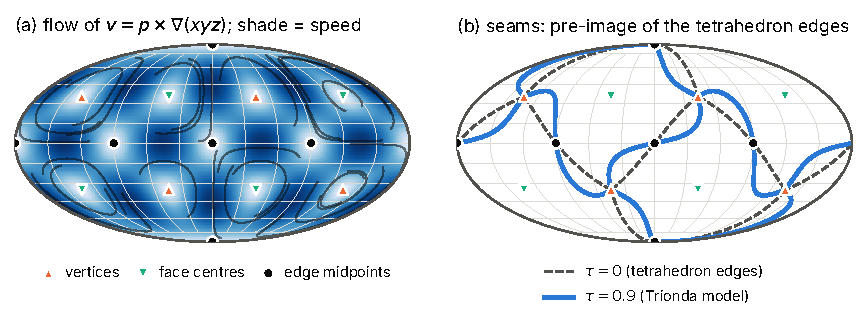
\includegraphics[width=\textwidth]{fig2_flow}
\caption{The flow behind the Trionda model. (a) Speed of $v=p\times\nabla(xyz)$ (shading) with a few flow lines and the 14 zeros.
(b) Seams of the straight tetrahedron (dashed) and their pre-images under $\Phi_{-\tau}$ for $\tau=\tauDefault$.}\label{fig:flow}
\end{figure}
\begin{figure}[tbp]
\centering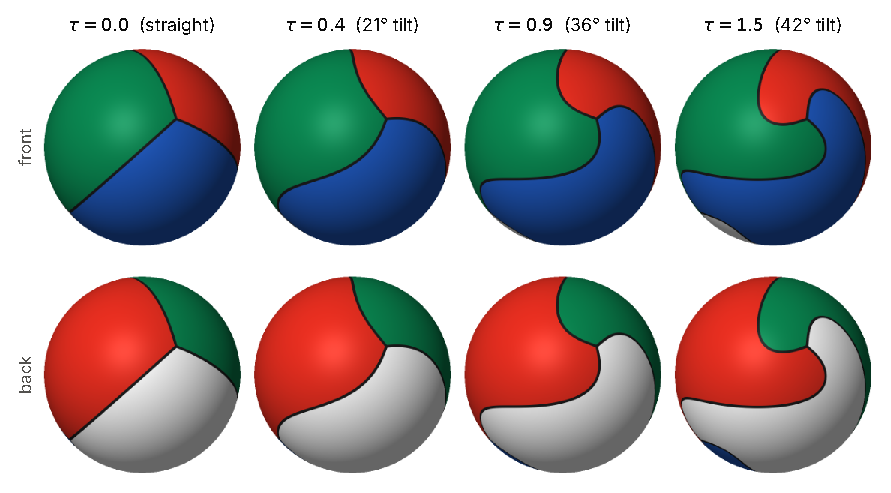
\includegraphics[width=\textwidth]{fig3_tau_sweep}
\caption{The model for increasing flow time $\tau$; the tilt in the titles is $\arctan\tanh\tau$ (\cref{prop:tilt}).
Front and back are two views of the same ball.}\label{fig:views}
\end{figure}

\subsection{Seam geometry at the fixed points}
\begin{proposition}[tilt at edge midpoints]\label{prop:tilt}
In the Trionda model the seam through each edge midpoint $m$ makes the angle $\alpha(\tau)=\arctan\tanh\tau$ with the straight edge.
\end{proposition}
\begin{proof}
By symmetry take $m=(1,0,0)$, with tangent coordinates $(y,z)$ and the straight edge along $y=z$ (it joins $\mathbf T_0$ and $\mathbf T_1$).
Near $m$, $\nabla f=(yz,z,y)$ and $v=(y^2-z^2,-y,z)$, so to first order $\dot y=-y$, $\dot z=z$. Hence $\Phi_{-\tau}(y,z)=(e^{\tau}y,e^{-\tau}z)+O(2)$,
and the seam is tangent at $m$ to $(e^{\tau},e^{-\tau})$. The angle between $(1,1)$ and $(e^\tau,e^{-\tau})$ has tangent
$\tan(\tfrac\pi4-\arctan e^{-2\tau})=\tanh\tau$.
\end{proof}
Since $\alpha\to45^\circ$ as $\tau\to\infty$, the seam can never rotate past $45^\circ$ at the midpoints. Numerically the tilt measured on the pulled-back
curves agrees with this formula (\cref{fig:tau}a).

\begin{proposition}[swirl at the vertices]\label{prop:vertex}
Near a tetrahedron vertex $\Phi_\tau$ is, to first order, a rotation about the vertex through the angle $2\tau/\sqrt3$ (clockwise seen from outside); near a
face centre it is the opposite rotation. The three seams still meet at $120^\circ$.
\end{proposition}
\begin{proof}
At $p_0=\mathbf T_0$ the ambient Hessian of $xyz$ is $\tfrac1{\sqrt3}(\mathbf 1\mathbf 1^{\!\top}-\mathrm{Id})$, which equals $-\tfrac1{\sqrt3}$ on tangent vectors, and
$p_0\cdot\nabla f=3f(p_0)=\tfrac1{\sqrt3}$. The Hessian of $f|_{\Sph}$ is the tangential block minus $(p_0\cdot\nabla f)\mathrm{Id}$, i.e.\ $-\tfrac2{\sqrt3}\mathrm{Id}$. Thus
$\nabla_{\!S}f\approx-\tfrac2{\sqrt3}\delta$ and $v\approx-\tfrac2{\sqrt3}\,p_0\times\delta$, a rigid rotation with rate $2/\sqrt3$. At $-p_0$ the sign of $f$ flips. Three-fold symmetry
keeps the seams $120^\circ$ apart.
\end{proof}
At $\tau=\tauDefault$ the vertex swirl is $\vertexAngleDefault^\circ$, and the seams cross the edge midpoints at $\tiltDefault^\circ$.
These two numbers, together with the straight edge length, essentially determine the look of one seam.

\begin{proposition}[chirality]\label{prop:chiral}
For $\tau\ne0$ the Trionda model is chiral: $\Sym(\mathcal P_\tau)=T$.
\end{proposition}
\begin{proof}
An isometry preserving the seam network permutes its vertices, the four trivalent points $\mathbf T_k$, hence lies in $T_d$ (the isometry group of the regular tetrahedron).
All rotations in $T$ are symmetries by \cref{thm:partition}(iii). If an improper element of $T_d$ were a symmetry, then so would be the reflection $r$ in the plane $\Pi$
through the centre and the edge $\mathbf T_0\mathbf T_1$ (their quotient lies in $T$). $r$ fixes $m=(1,0,0)$ and the edge direction, and reverses the sign of a tilt away from it.
But exactly one seam passes through $m$ and it is tilted by $\alpha\in(0,45^\circ)$ by \cref{prop:tilt}; $r$ would map it to a seam through $m$ tilted by $-\alpha$,
a different curve. Hence $r\notin\Sym(\mathcal P_\tau)$.
\end{proof}
For $\tau=0$ one recovers the achiral $T_d$ partition. The mirror image of the model for $\tau$ is the model for $-\tau$.

\begin{remark}[other groups]\label{rem:families}
\cref{thm:partition} holds for any $G$ and any $G$-invariant $f$. We use $f=x^4+y^4+z^4$ for the cube and octahedron ($O$) and $f=\sum_{a}(p\cdot a)^6$ over the six five-fold axes
$a$ for the dodecahedron and icosahedron ($I$). The flow is rescaled so the hyperbolic rate at an edge midpoint is $1$.
Only for $xyz$ does \cref{prop:tilt} take the closed form above: for the other invariants the achievable edge tilt saturates at $\limCube^\circ$ (cube),
$\limOcta^\circ$ (octahedron), $\limDodeca^\circ$ (dodecahedron) and $\limIcosa^\circ$ (icosahedron), against $\limTetra^\circ$ for the tetrahedron
(computed from the exact Jacobian). To compare families we therefore calibrate each one to the \emph{same} edge tilt of $\famTilt^\circ$ rather than the same $\tau$.
\end{remark}

%-------------------------------------------------------------------------------------------------------------
%-------------------------------------------------------------------------------------------------------------
\section{The Hat Trick ball}\label{sec:hat}
The \emph{hat} of \citet{smith_hat} is a polykite: eight kites glued edge to edge. It is a $13$-gon with six sides of length $1$, six of length $\sqrt3$ and one of length $2$ (two collinear unit edges); its interior angles are
$90^\circ$ (four times), $120^\circ$ (five times), $240^\circ$ (twice) and $270^\circ$ (twice), summing to $1980^\circ=(13-2)\cdot180^\circ$. It is chiral, and its area is $8\sqrt3$ for unit short edge, because a kite has area $\sqrt3$ (\cref{fig:hat}).
\begin{figure}[tbp]
\centering\includegraphics[width=0.45\textwidth]{hat_trick_hat}
\caption{The hat: eight kites, with edge lengths $1$ and $\sqrt3$ and one straight edge of length $2$.}\label{fig:hat}
\end{figure}

\subsection{The kite complex}
Take a triangulation of the sphere in which each triangle $t=(v_0,v_1,v_2)$ (counter-clockwise) is split into three kites around its centroid. Kite $3t+i$ belongs to vertex $v_i$, and its corners in order are $v_i$, the midpoint of $v_iv_{i+1}$,
the centroid of $t$, and the midpoint of $v_{i+2}v_i$. With triangulation edges of length $2\sqrt3$ and hexagon sides of length $2$, a kite has sides $\sqrt3,1,1,\sqrt3$, diagonals $2$ ($v$ to centroid) and $\sqrt3$ (midpoint to midpoint), and angles $60^\circ,90^\circ,120^\circ,90^\circ$ at $v$, midpoint, centroid and midpoint.
These are exactly the kites of the hat. We use the triangulation that is the dual of the Goldberg polyhedron $\mathrm{GP}(3,0)$ \citep{goldberg1937}: a frequency-$3$ subdivision of the icosahedron with \htTiles\ vertices, \htTriangles\ triangles, $12$ vertices of degree $5$ and $80$ of degree $6$.
The $12$ degree-$5$ vertices are not given kites; their kites (five each) are left out as \emph{pentagonal holes}. That leaves \htKites\ kites, i.e.\ exactly $60$ hats' worth.

\subsection{An exact, icosahedrally symmetric cover}
A \emph{placement} of the hat is a set of $8$ kites of the complex that is glued like the hat; we use orientation-preserving embeddings of the hat only (so every hat has the same hand). There are \htPlacements\ placements.
An \emph{exact cover} of the \htKites\ kites by placements is a tiling. We look for tilings invariant under the rotation group $I$ ($|I|=\htRotations$) by running Knuth's Algorithm~X over $I$-orbits of placements.
\begin{proposition}[the covers]\label{prop:covers}
There are exactly \htTilings\ tilings that are invariant under $I$; both consist of $60$ hats forming one free orbit of $I$, and each pentagon is touched by $5$ hats. Their two outlines share one $40$-kite patch type. We call them variants $0$ and $1$.
\end{proposition}
This is a statement about the exhaustive search (it ends with the search exhausted), not a hand proof. In particular, all hats in a tiling are images of one hat under $I$, so a hat has trivial stabiliser, which is the fact used in \cref{prop:free}.

\begin{figure}[tbp]
\centering\includegraphics[width=\textwidth]{hat_trick_ball}
\caption{The Hat Trick model (variant 0) after relaxation, looking down a 5-fold (pentagon), a 3-fold and a 2-fold axis. Hats are coloured so that neighbouring hats differ; the 12 pentagons are black.}\label{fig:hatball}
\end{figure}

\subsection{Flatness and the angle ledger}
\begin{proposition}[ledger of the flat hat model]\label{prop:hatledger}
At every corner of the kite complex the kite angles add up to $360^\circ$, except at the corners of the pentagonal holes. Each hole has $10$ corners: five centroids, with total angle $\theta_c=240^\circ$, and five edge midpoints,
with $\theta_m=180^\circ$, so the hole has curvature $K=360^\circ+180^\circ\cdot10-(5\cdot240^\circ+5\cdot180^\circ)=60^\circ$. Hence the total deficit is $12\times60^\circ=720^\circ$.
\end{proposition}
\begin{proof}
A vertex of degree $6$ is surrounded by $6$ kites with angle $60^\circ$, a centroid by $3$ kites with $120^\circ$, and an edge midpoint by $4$ kites with $90^\circ$ (two from each of the two adjacent triangles). Next to a degree-$5$ vertex $p$, the triangle at $p$ has only two of its three kites, giving $2\cdot120^\circ=240^\circ$ at its centroid, and the edge $pw$ has only the kites at $w$, giving $2\cdot90^\circ=180^\circ$ at its midpoint. We checked these totals on the actual complex:
of the $\htVerts$ kite-complex corners, $\htFlatCorners$ are flat, there are $\htCentroidCorners$ centroid corners with $240^\circ$ and $\htMidCorners$ midpoint corners with $180^\circ$ (all in the holes).
\end{proof}
So the flat model has no curvature except at the pentagons, $60^\circ$ each, which is the ledger of \cref{fig:ledger}; the Hat Trick is the spherical analogue of ``five hats around a pentagon'': in the flat model the five hats around a pentagon only fit together with a $60^\circ$ angular gap, and the sphere supplies exactly that.

\subsection{Relaxation on the sphere}
The flat hats do not fit exactly on the unit sphere, so we relax: least squares on all kite side and diagonal lengths with a common scale, plus straightness constraints on the hexagon edges ($=2$) and the triangulation edges ($=2\sqrt3$), all vertices on the unit sphere.
The result has an rms relative strain of \htRms\,\% and a maximum of \htMaxStrain\,\% over \htNConstraints\ constraints; hats are $\htAreaRatio$ times the area of a pentagon, and the hat areas differ by less than $\htAreaSpread$ (relative). All numbers in this paper use the relaxed model.
The strain is the price of fitting flat hats on a sphere; it also breaks the exact selection rule slightly (\cref{fig:spectra}).

\subsection{Why only frequency three?}\label{sec:freq}
The same construction works on the frequency-$f$ geodesic sphere for odd $f$ (with $f=n+1$), where the number of hats is $7.5(f^2-1)$, so $f=3$ gives $60$. We searched all of $f=3,5,7,9$ with Algorithm X over the orbits of several rotation subgroups,
from $I$ down to the trivial group (\cref{tab:hatfreq}).
\begin{table}[tbp]\centering\footnotesize
\begin{tabular}{@{}rrrrrrrr@{}}
\toprule
$f$ & tiles & hats & $I$ & $T$ & $C_5$ & $C_1$ & $C_1$, both hands \\
\midrule
3 & 92 & 60 & 2 & 2 & 16 & $\ge1000$ & $\ge1000$ \\
5 & 252 & 180 & 0 & 0 & 0 & 0 & 0 \\
7 & 492 & 360 & 0 & 0 & 0 & 0 & 0 \\
9 & 812 & 600 & 0 & 0 & 0 & 0 & $0^{*}$ \\
\bottomrule
\end{tabular}

\caption{Hat tilings of $\mathrm{GP}(f,0)$ with pentagonal holes, by the symmetry group imposed. An entry is the number of tilings found; ``$\ge$'' means the search was stopped at the limit without exhausting the space, and $0^{*}$ means it was stopped at the node limit without finding any tiling.}\label{tab:hatfreq}
\end{table}
For $f=3$ tilings exist and the $I$-invariant ones are exactly two. For $f=5,7,9$ the searches are exhaustive for every symmetry group tried, with the hat's hand fixed, and find none. With both hands allowed, $f=5$ and $f=7$ are exhausted with none, and $f=9$ was not exhausted at the node limit.
This covers only $\mathrm{GP}(f,0)$ with pentagon holes: the families $\mathrm{GP}(m,n)$ with $n>0$ are not tested, and no theorem is claimed.

%-------------------------------------------------------------------------------------------------------------
\section{Symmetry-restricted multipoles of the seam network}\label{sec:multipoles}
Let $\mu$ be arclength measure on the seam network, $a_{\ell m}=\int\overline{Y_{\ell m}}\,d\mu$, and
\begin{equation}
 Q_\ell=\sum_{m=-\ell}^{\ell}\frac{|a_{\ell m}|^2}{|a_{00}|^2},
\end{equation}
which is invariant under rotations of the ball and measures the strength of the degree-$\ell$ component of the seam density relative to its mean.

\begin{theorem}[selection rule]\label{thm:selection}
If $\mu$ is $G$-invariant then $(a_{\ell m})_m$ lies in the space $H_\ell^G$ of $G$-invariant harmonics of degree $\ell$, so $Q_\ell=0$ whenever $H_\ell^G=0$. Moreover
\begin{equation}
 \dim H_\ell^G=\frac1{|G|}\sum_{g\in G}\chi_\ell(g),\qquad \chi_\ell(\theta)=\frac{\sin\!\big((2\ell+1)\theta/2\big)}{\sin(\theta/2)},
\end{equation}
where $\theta$ is the rotation angle of $g$.
\end{theorem}
\begin{proof}
$\mu$ is $G$-invariant iff $\mu(\cdot)=\mu(g\,\cdot)$, which translates into $a_{\ell\bullet}$ being fixed by the irreducible representation of $SO(3)$ of degree $\ell$ restricted to $G$.
The dimension of the fixed space is the multiplicity of the trivial character \citep{serre_reps}, and $\chi_\ell$ is the character of that representation.
\end{proof}
\Cref{tab:inv} lists the dimensions \citep[cf.][]{stanley_invariants}. Since $T$, $O$, $I$ act irreducibly on $\R^3$ there is no invariant of degree $1$, and \cref{tab:inv} shows none of degree $2$ either, so $Q_1=Q_2=0$ for all of them: the seam network has its centre of mass at the
origin and an isotropic inertia tensor. The first non-trivial multipole is $\ell=3$ for $T$ (the cubic $xyz$ is itself such an invariant), $\ell=4$ for $O$ and $\ell=6$ for $I$.
This is one precise sense in which the tetrahedral layout is ``less symmetric'': its seam density departs from a uniform one already at degree~3, the icosahedral one only at degree~6.

\begin{table}[tbp]\centering\footnotesize
\begin{tabular}{@{}lrrrrrrrrrrrr@{}}
\toprule
$\ell$ & 1 & 2 & 3 & 4 & 5 & 6 & 7 & 8 & 9 & 10 & 11 & 12 \\
\midrule
$\dim H_\ell^{T}$ & 0 & 0 & 1 & 1 & 0 & 2 & 1 & 1 & 2 & 2 & 1 & 3 \\
$\dim H_\ell^{O}$ & 0 & 0 & 0 & 1 & 0 & 1 & 0 & 1 & 1 & 1 & 0 & 2 \\
$\dim H_\ell^{I}$ & 0 & 0 & 0 & 0 & 0 & 1 & 0 & 0 & 0 & 1 & 0 & 1 \\
\bottomrule
\end{tabular}

\caption{Dimension of the space of $G$-invariant spherical harmonics of degree $\ell$ (character formula).}\label{tab:inv}
\end{table}

\begin{proposition}[exposure filter]\label{prop:filter}
For a zonal kernel $K(p\cdot n)$ put $G(n)=\int K(p\cdot n)\,d\mu(p)$. By the Funk--Hecke theorem \citep{muller_harmonics}, $G=\sum_\ell\lambda_\ell\sum_ma_{\ell m}Y_{\ell m}$ with
$\lambda_\ell=2\pi\!\int_{-1}^1K(u)P_\ell(u)\,du$. If $K$ is even ($K(-u)=K(u)$) then $\lambda_\ell=0$ for odd $\ell$.
\end{proposition}
We use the Gaussian band $K(\theta)\propto\exp[-(\theta-\theta_s)^2/2\sigma^2]$ around a ``separation circle'' at angle $\theta_s$ from the flow axis $n$; $G(n)$ is then the seam length
near that circle, per radian, for a ball moving along $n$. It is a \emph{geometric proxy only}: it does not model the boundary layer. For $\theta_s=90^\circ$ the kernel is even, so for
this choice $G$ is constant up to degree $3$ for $T$ and $O$ \,(first variation at $\ell=4$) and up to degree $5$ for $I$ (first variation at $\ell=6$), in agreement with \cref{fig:expo}.

%-------------------------------------------------------------------------------------------------------------
\section{Numerical comparison}\label{sec:numerics}
We compare fourteen layouts: the straight tetrahedron, the cube, octahedron, dodecahedron and icosahedron and their chiral versions ($\famTilt^\circ$ edge tilt), the
Trionda model ($\tau=\tauDefault$ and $\famTilt^\circ$), the truncated icosahedron, and a Goldberg 42-panel ball (12 pentagons and 30 hexagons, centred on the vertices and edge midpoints of the icosahedron, with the pentagon plane height tuned so that all 42 panels have equal area) with its chiral version, obtained from the same icosahedral flow as the chiral icosahedron. All quantities are on the unit sphere. Symmetry groups are computed
numerically by testing which isometries map the panel partition to itself; seam length is computed exactly along the seam curves; $Q_\ell$ by quadrature on the seam curves; the exposure
coefficient of variation (CV) of $G$ over $3000$ near-uniform axes with $\theta_s=90^\circ$, $\sigma=10^\circ$.

\begin{table}[tbp]\centering\footnotesize
\begin{tabular}{@{}lrlrrrrr@{}}
\toprule
layout & panels & symmetry & seam length & length/area & $\ell^*$ & exposure CV & mean $|\kappa_g|$ \\
\midrule
tetra-4 & 4 & $T_d$ (12+12) & 11.46 & 0.912 & 3 & 0.186 & 0.00 \\
\textbf{Trionda model} ($\tau=0.9$) & 4 & $T$ (12) & 13.57 & 1.080 & 3 & 0.163 & 1.31 \\
Trionda model ($20^\circ$ tilt) & 4 & $T$ (12) & 11.86 & 0.944 & 3 & 0.184 & 0.72 \\
\addlinespace
cube-6 & 6 & $O_h$ (24+24) & 14.77 & 1.175 & 4 & 0.305 & 0.00 \\
cube-6, chiral & 6 & $O$ (24) & 15.44 & 1.229 & 4 & 0.293 & 1.32 \\
octa-8 & 8 & $O_h$ (24+24) & 18.85 & 1.500 & 4 & 0.260 & 0.00 \\
octa-8, chiral & 8 & $O$ (24) & 19.45 & 1.548 & 4 & 0.247 & 0.83 \\
\addlinespace
dodeca-12 & 12 & $I_h$ (60+60) & 21.89 & 1.742 & 6 & 0.174 & 0.00 \\
dodeca-12, chiral & 12 & $I$ (60) & 23.06 & 1.835 & 6 & 0.169 & 2.43 \\
\addlinespace
icosa-20 & 20 & $I_h$ (60+60) & 33.21 & 2.643 & 6 & 0.139 & 0.00 \\
icosa-20, chiral & 20 & $I$ (60) & 34.28 & 2.728 & 6 & 0.133 & 1.21 \\
\addlinespace
goldberg-42 (12 pent., 30 hex.) & 42 & $I_h$ (60+60) & 42.52 & 3.383 & 6 & 0.027 & 0.00 \\
goldberg-42, chiral & 42 & $I$ (60) & 43.30 & 3.446 & 6 & 0.025 & 0.76 \\
\addlinespace
classic-32 (trunc.\ icosahedron) & 32 & $I_h$ (60+60) & 36.57 & 2.910 & 6 & 0.056 & 0.00 \\
\bottomrule
\end{tabular}

\caption{Fourteen layouts. ``Symmetry'' lists the group and the number of rotations (plus improper isometries if achiral). $\ell^*$: lowest $\ell\ge1$ with $Q_\ell>10^{-9}$.
Length/area is seam length divided by $4\pi$. Mean $|\kappa_g|$ is the arclength-weighted mean geodesic curvature of the seams.}\label{tab:family}
\end{table}

\paragraph{Symmetry and multipoles.}
In every row, the detected rotation count equals the order of the intended group ($12$, $24$ or $60$), the chiral variants have no improper symmetry, and the straight ones have as many
improper as proper symmetries. This confirms \cref{thm:partition}(iii) and \cref{prop:chiral} and also validates the code. The numerically computed multipoles satisfy
\cref{thm:selection} exactly: $Q_\ell<10^{-9}$ whenever $\dim H_\ell^G=0$, and in all fourteen cases $\ell^*$ equals the first degree with $\dim H^G_\ell>0$ (\cref{fig:multi}). The classic ball and the Trionda model are separated by $\ell^*=6$ versus $3$.

\begin{figure}[tbp]
\centering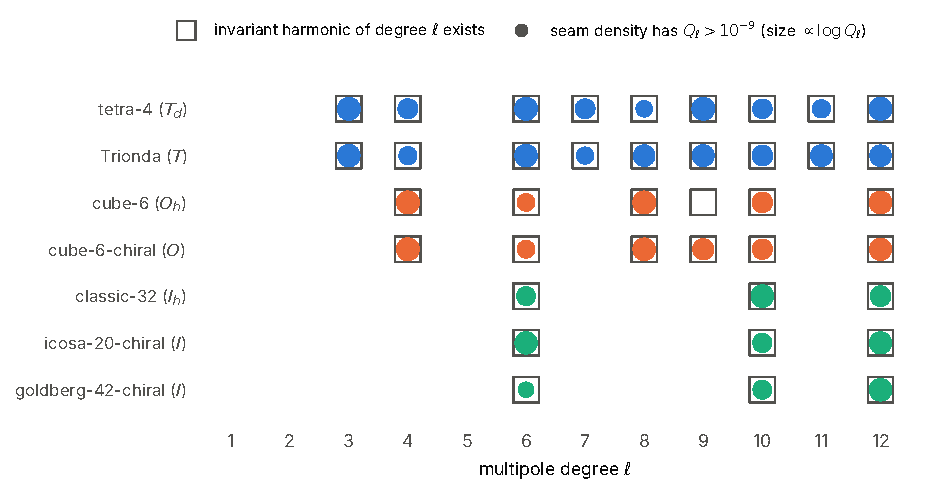
\includegraphics[width=0.82\textwidth]{fig6_multipoles}
\caption{Which multipoles $Q_\ell$ of the seam density are nonzero. Squares: an invariant harmonic of degree $\ell$ exists for the group. Dots: $Q_\ell>10^{-9}$.
There is no dot without a square, and chirality does not change the pattern within a group.}\label{fig:multi}
\end{figure}

\paragraph{Seams.}
The straight tetrahedron needs the least seam per unit area of any layout in \cref{tab:family} \,(\straightL\ in total). At $\tau=\tauDefault$ the Trionda model has
\LDefault, i.e.\ \LPctDefault\,\% more seam than the straight edges, and a mean geodesic curvature of \kgMeanDefault; seam length grows monotonically with $\tau$ (\cref{fig:tau}b), reaching a factor
\LRatioTauTwo\ at $\tau=2$.

\begin{figure}[tbp]
\centering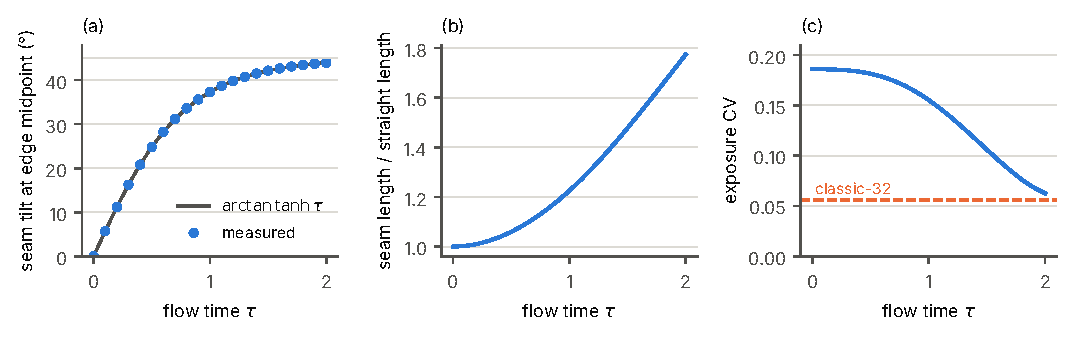
\includegraphics[width=\textwidth]{fig5_tau_dependence}
\caption{Dependence on the flow time $\tau$ for the Trionda model. (a) Tilt of the seam at the edge midpoint, measured on the pulled-back curve, against $\arctan\tanh\tau$.
(b) Seam length relative to the straight edges. (c) Exposure CV; the dashed line is the truncated icosahedron.}\label{fig:tau}
\end{figure}

\paragraph{Exposure proxy.}
\Cref{fig:expo} shows $G(n)/\bar G$ for four layouts, and the last columns of \cref{tab:family} give the CV. At the default proxy parameters three observations hold:
(i) chirality lowers the CV in all six straight/chiral pairs of \cref{tab:family}, though only slightly at the matched $\famTilt^\circ$ tilt (for the tetrahedron $\expTetra\to\expTrionTwenty$);
(ii) for the tetrahedron the CV falls steadily with $\tau$, from $\expTetra$ to $\expTrionda$ at $\tau=\tauDefault$ and $\expTauTwo$ at $\tau=2$ (\cref{fig:tau}c);
(iii) the layouts with the most panels have the lowest CV: the Goldberg ball ($\expGoldberg$, chiral $\expGoldbergChiral$) is lowest, the truncated icosahedron next ($\expClassic$, about $\expRatioClassic$ times lower than the Trionda model at $\tau=\tauDefault$); within the $I_h$ layouts of \cref{tab:family} the CV decreases with the panel count ($12$, $20$, $32$, $42$ panels). Four values do not make a trend, and we draw no further conclusion.

\begin{figure}[tbp]
\centering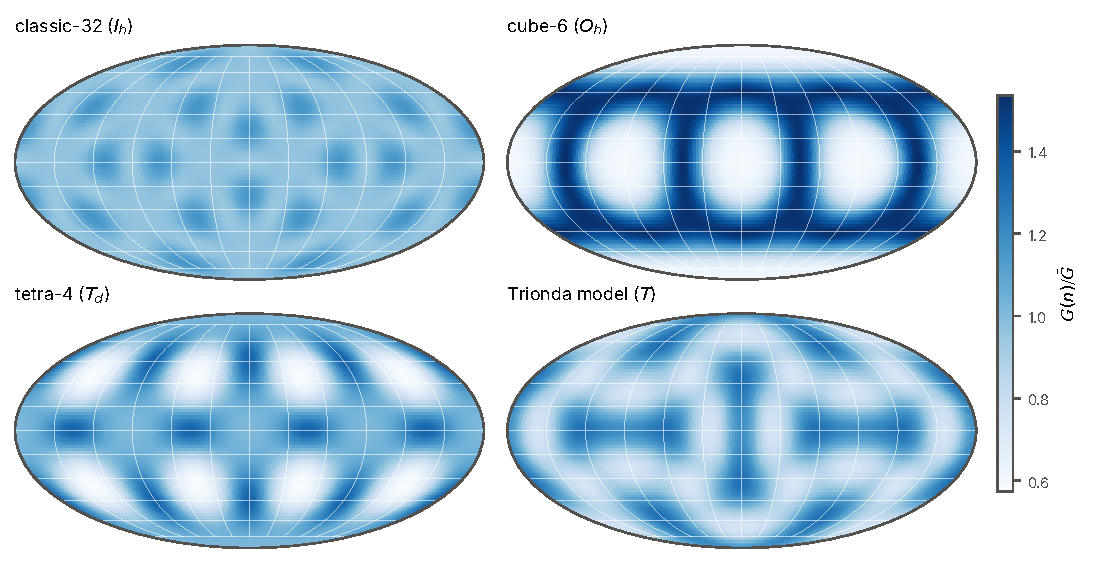
\includegraphics[width=\textwidth]{fig7_exposure_maps}
\caption{Exposure $G(n)/\bar G$ over all flow directions $n$ ($\theta_s=90^\circ$, $\sigma=10^\circ$; shared colour scale). The cube concentrates exposure around three great circles, the
tetrahedral layouts around the axes through edge midpoints, the truncated icosahedron is nearly uniform.}\label{fig:expo}
\end{figure}

\paragraph{Sensitivity.}
The proxy has two free parameters, so we checked how conclusions depend on them (\cref{tab:sens}; $\theta_s\in\{70^\circ,\dots,120^\circ\}$, $\sigma\in\{5^\circ,10^\circ,15^\circ\}$, 18 combinations).
Robust across all 18: the Trionda model has lower CV than the straight tetrahedron; $\tau=2$ is lower than $\tau=\tauDefault$; and the truncated icosahedron is lower than the Trionda model.
\emph{Not} robust: the ordering of the cube and the tetrahedron reverses with $\theta_s$ (at $\theta_s=90^\circ$ the cube is worse, at $70^\circ$ and $110^\circ$ it is better). We therefore draw no conclusion about
cube versus tetrahedron.

\begin{table}[tbp]\centering\footnotesize
\begin{tabular}{@{}lrrrrrr@{}}
\toprule
separation angle $\theta_s$ & $70^\circ$ & $80^\circ$ & $90^\circ$ & $100^\circ$ & $110^\circ$ & $120^\circ$ \\
\midrule
classic-32 & 0.045 & 0.019 & 0.056 & 0.019 & 0.045 & 0.048 \\
cube-6 & 0.097 & 0.208 & 0.305 & 0.208 & 0.097 & 0.218 \\
tetra-4 & 0.350 & 0.233 & 0.186 & 0.233 & 0.350 & 0.409 \\
Trionda model ($\tau=0.9$) & 0.299 & 0.187 & 0.163 & 0.187 & 0.299 & 0.341 \\
Trionda model ($\tau=2$) & 0.214 & 0.129 & 0.063 & 0.129 & 0.214 & 0.232 \\
\bottomrule
\end{tabular}

\caption{Exposure CV against the separation angle $\theta_s$ ($\sigma=10^\circ$).}\label{tab:sens}
\end{table}

%-------------------------------------------------------------------------------------------------------------
%-------------------------------------------------------------------------------------------------------------
\section{Comparing the two balls}\label{sec:compare}
\Cref{tab:compare} puts the two models next to the classical layouts, computed with the same tools as \cref{tab:family} (seam length by quadrature on the seams, $Q_\ell$ with $\ell^*$ the lowest $\ell\ge1$ with $Q_\ell>10^{-9}$,
the exposure proxy of \cref{sec:multipoles} over $2000$ near-uniform axes).
\begin{table}[tbp]\centering\footnotesize
\begin{tabular}{@{}lrlrrrr@{}}
\toprule
layout & panels & group & seam length & $\ell^*$ & exposure CV & mean $|\kappa_g|$ \\
\midrule
\textbf{Trionda model} ($\tau=0.9$) & 4 & $T$ & 13.57 & 3 & 0.1628 & 1.31 \\
tetra-4 & 4 & $T_d$ & 11.46 & 3 & 0.1859 & 0.00 \\
\textbf{Hat Trick}, tiling 0 & 72 & $I$ & 72.02 & 6 & 0.0089 & 0.00 \\
Hat Trick, tiling 1 & 72 & $I$ & 71.32 & 6 & 0.0136 & 0.00 \\
icosa-20 & 20 & $I_h$ & 33.21 & 6 & 0.1389 & 0.00 \\
classic-32 & 32 & $I_h$ & 36.57 & 6 & 0.0559 & 0.00 \\
goldberg-42 & 42 & $I_h$ & 42.52 & 6 & 0.0269 & 0.00 \\
\bottomrule
\end{tabular}

\caption{The Trionda and the Hat Trick against the classical layouts. The two Hat Trick rows are the two $I$-invariant tilings. The exposure CVs here use $2000$ axes, so they differ slightly in the third digit from \cref{tab:family}, which uses $3000$.}\label{tab:compare}
\end{table}
Three points stand out.
\begin{enumerate}
\item \textbf{Seams.} The Hat Trick has \cmpSeamRatio\ times the seam length of the Trionda (\cmpHatSeam\ against \cmpTriSeam), because it has $72$ panels against $4$; its panels are far from round (isoperimetric quotient \cmpHatShape\ for hats against \cmpPentShape\ for pentagons, where a disc has $1$).

\item \textbf{Multipoles.} $\ell^*=\cmpTriLow$ for the Trionda and $\cmpHatLow$ for the Hat Trick, as predicted in \cref{sec:connections}.
\item \textbf{Exposure.} The Hat Trick has the lowest CV of any layout in the table (\cmpHatCV, \cmpHatCVone\ for the second tiling) against \cmpTriCV\ for the Trionda, a ratio of \cmpRatioCV. The Goldberg-42 ball ($\cmpGoldCV$) and the truncated icosahedron ($\cmpClassicCV$) are
in between. Within the sensitivity limits of \cref{sec:numerics} this is a statement about a geometric proxy, not about aerodynamics.
\end{enumerate}
\begin{figure}[tbp]
\centering\includegraphics[width=\textwidth]{compare_exposure}
\caption{Exposure maps over all flow axes for the Trionda (left, in the Hat Trick's frame) and the Hat Trick (middle), on one colour scale, and their histograms (right). The maps use a regular longitude--latitude grid of axes, so the CVs in their titles
differ slightly from \cref{tab:compare}, which samples random axes.}\label{fig:exposure2}
\end{figure}

%-------------------------------------------------------------------------------------------------------------
\section{Mixing the two}\label{sec:blend}
Because $T\subset I$ (\cref{prop:oneframe}), two natural hybrids exist.

\subsection{Hat-Trionda: four panels made of hats}
Place the Trionda in the Hat Trick's frame and assign every hat and every pentagon to the Trionda panel that contains most of its area (area measured by sampling each kite on a $5\times5$ grid).
\begin{proposition}[Hat-Trionda]\label{prop:hattrionda}
If the assignment is well defined (no ties), it is $T$-equivariant, and each of the four Trionda panels receives exactly $15$ hats and $3$ pentagons.
\end{proposition}
\begin{proof}
Both the hat tiling and the Trionda are $T$-invariant, so $g\in T$ maps a hat to a hat and a panel to a panel, and the area of a hat in a panel equals the area of its image in the image panel. Hence the assignment $a$ from hats to panels satisfies $a(gh)=g\,a(h)$.
The group $T$ acts transitively on the four panels, so the fibres of an equivariant map all have the same size, namely $60/4=15$ for hats and $12/4=3$ for pentagons (the actions are free by \cref{prop:free}).
\end{proof}
In the model, every hat has a strict majority: the smallest majority fraction is \blMinMaj\,\%, so there are no ties and the proposition applies. The result is shown in \cref{fig:hattrionda}. The seams between the four hat clusters have total length \blSeam\ (against \cmpTriSeam\ for the smooth Trionda), \blStraddle\ of the $60$ hats straddle a panel boundary, and \blMismatch\,\% of the sphere's area lies in a different panel than the smooth Trionda would put it.
\begin{figure}[tbp]
\centering\includegraphics[width=\textwidth]{compare_hat_trionda}
\caption{Hat-Trionda. Left: the Trionda along a 3-fold (top) and a 2-fold (bottom) axis. Middle: hats and pentagons coloured by the Trionda panel that holds most of their area; every panel holds 15 hats and 3 pentagons. Right: where a hat sticks out of its panel (red; darker means more).}\label{fig:hattrionda}
\end{figure}

\subsection{The flow blend: the Hat Trick through the Trionda flow}
The flow $\Phi_\tau$ of \cref{sec:B} commutes with $T$ (\cref{lem:flow}(b)). Applying $\Phi_{-\tau}$ to the Hat Trick's seams, with the flow written in the shared frame, therefore gives a $T$-invariant network, still a tiling of the sphere by $72$ panels of the same areas as before (area preservation), but no longer $I$-invariant.
At $\tau=0$ it is the Hat Trick, and the sign of $\tau$ matters because the hat network is not exactly its own mirror image.
\begin{table}[tbp]\centering\footnotesize
\begin{tabular}{@{}rrrrrr@{}}
\toprule
$\tau$ & seam length & exposure CV & $\ell^*$ & $Q_3$ & $Q_4$ \\
\midrule
$-0.9$ & 82.96 & 0.0424 & 3 & $3.2\times10^{-4}$ & $2.0\times10^{-2}$ \\
$-0.6$ & 77.03 & 0.0216 & 3 & $1.7\times10^{-4}$ & $3.6\times10^{-3}$ \\
$-0.3$ & 73.30 & 0.0109 & 3 & $3.7\times10^{-5}$ & $9.1\times10^{-5}$ \\
$0.0$ & 72.02 & 0.0089 & 6 & $2.7\times10^{-18}$ & $4.6\times10^{-17}$ \\
$+0.3$ & 73.31 & 0.0135 & 3 & $9.6\times10^{-6}$ & $8.2\times10^{-4}$ \\
$+0.6$ & 77.09 & 0.0289 & 3 & $6.8\times10^{-6}$ & $7.9\times10^{-3}$ \\
$+0.9$ & 83.14 & 0.0500 & 3 & $8.5\times10^{-9}$ & $2.9\times10^{-2}$ \\
\bottomrule
\end{tabular}

\caption{The Hat Trick pushed through the Trionda flow for flow time $\tau$ (the Trionda uses $\tau=\tauDefault$). $\ell^*$ is the lowest $\ell\ge1$ with $Q_\ell>10^{-9}$.}\label{tab:flow}
\end{table}
\begin{figure}[tbp]
\centering\includegraphics[width=\textwidth]{compare_flow}
\caption{The flow blend. Top: the Hat Trick through the Trionda flow at $\tau=-0.9$, $0$ and $0.9$ (pentagons are black). Bottom: $Q_3$, the seam length, and the exposure CV against $\tau$.}\label{fig:flowblend}
\end{figure}
\Cref{tab:flow} and \cref{fig:flowblend} show three effects. (i) For every $\tau\ne0$ in the table, $\ell^*=3$: the harmonic that $I$ forbids and $T$ allows switches on, consistent with the symmetry dropping from $I$ to $T$ (\cref{thm:selection}). (ii) The seam length grows from \flSeamZero\ to \flSeamEnd\ at $\tau=0.9$, and the exposure CV from \flCVZero\ to \flCVEnd.
(iii) The blend therefore costs a little of the Hat Trick's uniformity, but even at $\tau=0.9$ its CV is \flRatio\ times lower than the Trionda's.
The power $Q_3$ is not monotone in $\tau$ (\cref{tab:flow}); it is small throughout, and we do not interpret the trend.

%-------------------------------------------------------------------------------------------------------------
\section{Discussion and limitations}
\paragraph{What we found.}
The Trionda and the Hat Trick are related by a single inclusion, $T\subset I$. It gives a shared frame, free actions with counts $4\to12\to72$, hybrids with exactly $15$ hats and $3$ pentagons per tetrahedral panel, a common curvature ledger
($720^\circ$ on $4$ or $12$ axes), and different multipole selection rules ($\ell^*=3$ against $6$). The geometric exposure proxy separates them by a factor of about \cmpRatioCV, with the Hat Trick close to uniform. The Trionda's reported properties---four panels, tetrahedral origin, curved and meandering seams, $12$ rotational symmetries---are realised by the model for any $\tau\ne0$, and the
count of $12$ is \emph{derived} (it is $|T|$) rather than assumed.

\paragraph{Symmetry and predictability.}
\citet{hasson_sciam} reports concern among experts that fewer symmetries may make a ball's flight less predictable at low spin. Our results quantify two purely geometric aspects:
the symmetry order ($12$ against $60$) and the order $\ell^*$ at which the seam density first departs from uniformity ($3$ against $6$). We also find that, within the Trionda model, a
chiral twist reduces the variation of the exposure proxy at the cost of longer and more curved seams, which is \emph{consistent with} meandering seams being a way of compensating for
the lower symmetry; this is a hypothesis, not something our computations show about the real design. The Hat Trick reaches an even lower proxy variation with its many small panels, at the price of much more seam.

\paragraph{Limitations.}
(1) Neither model is the manufacturer's geometry. The Trionda's seam curves, depth and surface texture are not described in the sources we use, and the real ball may deviate from exact $T$ symmetry (for example by the debossed icons or the embedded sensor, both reported by \citet{wiki_trionda}). The Hat Trick model is our reconstruction from a verbal description (hats around pentagons, 12 clusters, 72 panels): it is one of exactly two $I$-invariant solutions on $\mathrm{GP}(3,0)$, relaxed with rms edge strain of \htRms\,\% (maximum \htMaxStrain\,\%), so a real ball would differ in detail. The frequency scan covers only $\mathrm{GP}(f,0)$.
(2) The exposure proxy is not validated against flow data; it ignores seam depth, surface texture, spin and Reynolds number. (3) The Trionda flow depends on the choice of invariant $f$; $xyz$ is the simplest
one for $T$ but not the only one. (4) Family comparisons depend on how chirality is calibrated; we used equal edge tilt. (5) Sampling
error: exposure CV is estimated from $2000$--$3000$ axes, and $Q_\ell$ and seam lengths from quadrature on the seam curves, whose errors are far below the differences between the two balls, but not below the effects of the flow blend on $Q_3$, which we do not interpret.
(6) Hat-Trionda assigns whole hats by majority area, so it is a combinatorial hybrid, not a smooth interpolation. (7) The chirality measure depends on the sampling and on which improper isometries are tried.

\paragraph{Open questions.}
Why is the Hat Trick's seam network nearly mirror-symmetric although the hat is chiral? Which hat tiling and placement lie best inside the Trionda panels (rather than majority assignment)? Does the frequency scan change for $\mathrm{GP}(m,n)$ with $n>0$? Which $T$-equivariant four-panel partitions minimise seam length for a prescribed seam tilt, and can the true Trionda outline be matched by choosing $f$? How well does the exposure proxy correlate with wind-tunnel
measurements, which \citet{hasson_sciam} reports are planned?

\appendix
%-------------------------------------------------------------------------------------------------------------
\section{The barycentric construction and why it fails}\label{sec:A}
Let $V_0,V_1,V_2\in\R^2$ be the vertices of an equilateral triangle with circumradius $1$ (edge length $\sqrt3$,
height $3/2$). Edge $k$ runs from $V_k$ to $V_{k+1}$ with unit normal $\hat n_k$ pointing into the triangle. Deform it to
\begin{equation}\label{eq:chiral-edge}
 \mathbf c_k(t)=V_k+t(V_{k+1}-V_k)+\sqrt3\,\bigl(A\sin2\pi t+B\sin4\pi t\bigr)\hat n_k,\qquad t\in[0,1].
\end{equation}
The three deformed edges bound a three-armed ``boomerang'' $\Omega\subset\R^2$. Any odd function of $t-\tfrac12$ may replace the sine
profile. Each point of $\Omega$ has barycentric coordinates $w=(w_0,w_1,w_2)$, $\sum w_a=1$ with respect to $V$. For a
tetrahedron face $f=(\mathbf T_{i},\mathbf T_{j},\mathbf T_{k})$ define the fold
\begin{equation}\label{eq:fold}
 \Phi_f(w)=\frac{w_0\mathbf T_i+w_1\mathbf T_j+w_2\mathbf T_k}{\lVert w_0\mathbf T_i+w_1\mathbf T_j+w_2\mathbf T_k\rVert},
\end{equation}
and let $\Omega_f=\Phi_f(\Omega)$. We call $\{\Omega_f\}_f$ over the four faces \emph{Construction~A}.

\begin{proposition}[flat symmetry]\label{prop:flat}
Each deformed edge is point-symmetric about its midpoint $M_k$: $\mathbf c_k(1-t)=2M_k-\mathbf c_k(t)$.
\end{proposition}
\begin{proof}
The profile $g(t)=\sqrt3(A\sin2\pi t+B\sin4\pi t)$ satisfies $g(1-t)=-g(t)$, and the straight part satisfies
$V_k+(1-t)\Delta=2M_k-(V_k+t\Delta)$ with $\Delta=V_{k+1}-V_k$.
\end{proof}

Proposition~\ref{prop:flat} is exactly what one needs in the \emph{plane}: two copies of the panel unfolded across an edge fit. But the
fold \eqref{eq:fold} is not an isometry, and the point symmetry is not preserved:

\begin{proposition}[boundary mismatch]\label{prop:mismatch}
Let faces $f=(\mathbf T_i,\mathbf T_j,\mathbf T_k)$ and $f'=(\mathbf T_j,\mathbf T_i,\mathbf T_{k'})$ share the edge
$\{\mathbf T_i,\mathbf T_j\}$ (so that $\mathbf T_k+\mathbf T_{k'}=-(\mathbf T_i+\mathbf T_j)$). Let $u\in[0,1]$ be the position along the shared
edge measured from $\mathbf T_i$ and $c(u)=g(u)/(3/2)$ the barycentric offset of the boundary. Then the boundary points of
$\Omega_f$ and $\Omega_{f'}$ at position $u$ lie on the same ray from the origin if and only if $c(u)=0$.
\end{proposition}
\begin{proof}
A boundary point at position $u$ displaced by $c$ towards the interior has barycentric weights $(1-u-\tfrac c2,\,u-\tfrac c2,\,c)$,
since the unit normal is parallel to $V_k-\tfrac12(V_i+V_j)$. On $f$ this gives the unnormalised point
$P=(1-u-\tfrac c2)\mathbf T_i+(u-\tfrac c2)\mathbf T_j+c\,\mathbf T_k$. On $f'$ the same boundary is traversed from $\mathbf T_j$ with
parameter $1-u$, and the offset there is $g(1-u)/(3/2)=-c$, so the point is
$P'=(u+\tfrac c2)\mathbf T_j+(1-u+\tfrac c2)\mathbf T_i-c\,\mathbf T_{k'}
=(1-u+\tfrac{3c}2)\mathbf T_i+(u+\tfrac{3c}2)\mathbf T_j+c\,\mathbf T_k$. The vectors $\mathbf T_i,\mathbf T_j,\mathbf T_k$ are linearly independent;
their coordinate sums are $1$ for $P$ and $1+4c$ for $P'$. If $P'=\lambda P$ with $\lambda>0$ and $c\neq0$, the $\mathbf T_k$-coordinate
forces $\lambda=1$ and the sum forces $c=0$, a contradiction.
\end{proof}

Proposition~\ref{prop:mismatch} compares equal parameters $u$ only; it does not by itself prove that the two curves differ as sets, so
we measure the consequence directly. We sample $4\times10^5$ near-uniform points of $\Sph$ and count in how many of the four
panels each lies (\cref{fig:A}).

\begin{figure}[tbp]
\centering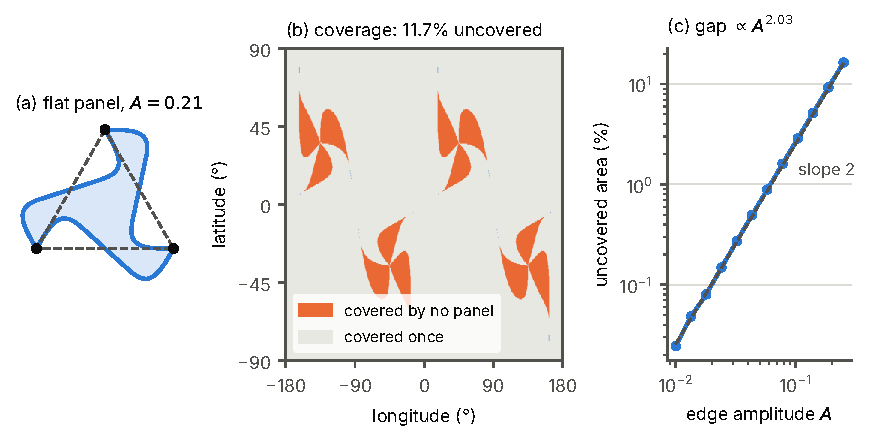
\includegraphics[width=\textwidth]{fig1_construction_A}
\caption{Audit of Construction~A. (a) The flat panel for $A=0.21$, $B=0.035$ and the reference triangle.
(b) Points of the sphere covered by none of the four folded panels (orange); overlaps are below $0.03\,\%$ and not visible.
(c) Uncovered area as a function of the amplitude $A$ (with $B=A/6$), log--log; the dashed line has slope~2.}\label{fig:A}
\end{figure}

\begin{itemize}
\item At $A=0.21$, $B=0.035$, \gapUser\,\% of the sphere is covered by no panel; overlaps are negligible.
\item For $A\le0.25$ the uncovered fraction follows a power law with fitted exponent \gapSlope, i.e.\ it is a second-order effect in the
 amplitude, consistent with the mismatch in the proof above being along the seam to first order.
\item At $A=0$ the construction is exact (it is the straight tetrahedron).
\end{itemize}
Construction~A therefore gives a faithful picture of the \emph{shape} of one panel in the plane, but not an exact closed ball.

%-------------------------------------------------------------------------------------------------------------
\section{A side study: folding patches of the Spectre monotile into spheres}\label{sec:spectre}
The \emph{Spectre} \citep{smith_spectre} is a chiral aperiodic monotile: a single polygon with $14$ edges whose tilings of the plane are all
non-periodic. This section asks a question that is independent of the ball model but
close in spirit to the hexagonal grids of \cref{fig:chiralhex}: \emph{which patches of this tile can be folded shut into a closed ball, and what is left
over when they cannot?} We use the straight-edged equilateral polygon (all $14$ edges of length $1$; the $a=b=1$ member of the family) and make no
claim about any real ball. The code is in \texttt{spectre/} of the repository, and every number below is produced by \texttt{make\_spectre\_data.py}.

\subsection{Folds, cones and holes}
All corner angles of the tile are multiples of $30^\circ$: $(90,120,270,120,90,120,270,120,180,120,90,240,90,240)$ in degrees, summing to $2160^\circ$.
Take a patch of $N$ tiles that is a topological disc, with boundary loop of $m$ unit edges. A \emph{fold} glues boundary edges in pairs, without crossing and
without changing any edge length, so the result is a surface that is flat except at vertices. Tiles are allowed to crease: they stay intrinsically flat.
At a vertex where several tile corners meet, the \emph{angle} is their sum $a$; if the vertex is closed (surrounded by tiles) its \emph{deficit} is $\delta=360^\circ-a$, which must be $\ge 0$ here.
Boundary loops that are left unglued are \emph{holes}. A hole with $n$ unit edges and total tile angle $\theta_i$ at its $i$th corner has interior angles $\alpha_i=360^\circ-\theta_i$ and
\emph{curvature}
\begin{equation}K\;=\;\sum_i\alpha_i-(n-2)\,180^\circ\;=\;360^\circ+180^\circ\,n-\sum_i\theta_i,\label{eq:holeK}\end{equation}
the amount of curvature a cap would have to carry; $K=0$ with a closing equilateral polygon (for example $n=6$, all $\alpha_i=120^\circ$) means the hole could be filled flat.

\begin{proposition}[angle ledger]\label{prop:ledger}
For a fold of a disc patch with $h$ holes (each a simple loop), $\sum_{\text{closed vertices}}\delta_v+\sum_{\text{holes}}K_j=720^\circ$.
\end{proposition}
\begin{proof}
Let $c$ be the number of closed vertices, $g$ the number of glued pairs and $H=\sum_j n_j$ the number of hole edges. Counting tile edges, $14N=2g+H$; the surface has $V=c+H$ vertices, $E=g+H$ edges and $F=N$
faces, and is a sphere with $h$ discs removed, so $V-E+F=2-h$, i.e.\ $c+N-g=2-h$. The tile angles add to $2160^\circ N$, and they are distributed over the closed vertices and the hole corners:
$\sum_v a_v+\sum_{j,i}\theta_{j,i}=2160^\circ N$. Hence $\sum_v(360^\circ-a_v)+\sum_j K_j=360^\circ c+360^\circ h+180^\circ H-2160^\circ N=360^\circ(c+h+H/2-6N)=360^\circ(c+N-g+h)=720^\circ$, using $g=7N-H/2$.
\end{proof}

\begin{lemma}[parity]\label{lem:parity}
The total number of hole edges is even. In particular a single hole cannot have an odd number of sides; pentagonal holes can occur only together with another odd hole.
\end{lemma}
\begin{proof}
The boundary of the patch has $m=14N-2g_0$ edges, and every glued pair removes two of them.
\end{proof}

A fold of a patch into a \emph{closed} ball has $h=0$, so its deficits are all $\ge0$ and sum to $720^\circ$. By Alexandrov's gluing theorem \citep{alexandrov_polyhedra}, such a polyhedral metric on the sphere is the boundary of a unique convex polyhedron, possibly degenerate, so the intrinsic folds below are realisable in space, with the tiles bent along creases.
The three-dimensional pictures in this section are \emph{not} that polyhedron: they come from a numerical relaxation (positions of the glued vertices with every tile-triangle edge kept at its length and a weak pull towards a sphere), whose residual edge strain is nonzero.

\subsection{An exact search over gluings}
Index the boundary edges cyclically $0,\dots,m-1$ and let $A_k$ be the total tile angle at the vertex between edges $k-1$ and $k$. Gluing edge $i$ to edge $j$ (reversed) identifies vertex $i+1$ with vertex $j$ and vertex $j+1$ with vertex $i$.
\begin{lemma}[runs]\label{lem:runs}
Let a run of edges $l,\dots,r$ be matched among themselves without crossings, with outermost pairs $(l_1,j_1),\dots,(l_s,j_s)$, where $l_1=l$, $l_{t+1}=j_t+1$ and $j_s=r$. Then vertices $l$ and $r+1$ become one vertex, whose share of the angle from the run is
$S+A_{r+1}$ with $S=A_{l_1}+\dots+A_{l_s}$, and the pair $(l_t,j_t)$ closes a vertex of angle $S_t+A_{j_t}$, where $S_t$ is the corresponding sum for the run strictly inside the pair.
A hole with reserved edges $r_1<\dots<r_k$ inside a glued pair $(l,j)$, with the gaps $G_0,\dots,G_k$ between them matched in runs, has corner angles
$\theta_{r_t}=S(G_{t-1})+A_{r_t}$ for $t\ge2$ and $\theta_{r_1}=S(G_0)+S(G_k)+A_{r_1}+A_j$.
\end{lemma}
\noindent(Induction on the number of pairs; each glued pair merges the two vertex pairs named above.) All angles are multiples of $30^\circ$ and at most $360^\circ$, so the achievable sums $S$ of a run are a $13$-bit mask, and an interval dynamic programme over runs
decides in $O(m^3)$ word operations whether a given gluing pattern exists (\texttt{spectre/dp.py}). For one hole the programme is run on the doubled loop, which covers every rotation and therefore \emph{every} non-crossing gluing. For several holes it covers the gluings in which each hole lies inside a glued pair and no hole is nested in another hole's region; a negative answer for two or more holes is a statement about that class only.

\emph{Validation.} For one tile ($m=14$) an exhaustive enumeration of all layouts of four reserved edges and all zip orders gives \spBruteOne\ reachable corner multisets, exactly those found by the programme; for six reserved edges the enumeration gives \spBruteSix, and for two tiles ($m=22$) and four reserved edges \spBruteTwo, and the programme finds all of them. Every fold the programme returns is replayed through an independent bookkeeping of vertices and angles, and \cref{prop:ledger} is asserted on it.

\subsection{What the search finds}
\paragraph{Closed balls.}
\Cref{tab:spclosure} gives, for random connected patches of $N$ tiles (up to \spPerN\ draws per size, from a Spectre patch), the fraction whose whole boundary can be glued shut. Small patches usually can; the fraction falls quickly
with $N$, from about $89\%$ at $4$ tiles to $5\%$ at $12$ and under $1\%$ at $20$ and $24$, but closed balls still exist at $19$--$21$ tiles (\cref{fig:spclosed}).
\begin{table}[tbp]\centering\footnotesize
\begin{tabular}{@{}rrrr@{}}
\toprule
tiles $N$ & patches & close up & \% \\
\midrule
4 & 150 & 133 & 88.7 \\
5 & 150 & 100 & 66.7 \\
6 & 150 & 68 & 45.3 \\
8 & 148 & 29 & 19.6 \\
10 & 149 & 14 & 9.4 \\
12 & 148 & 8 & 5.4 \\
16 & 141 & 0 & 0.0 \\
20 & 137 & 1 & 0.7 \\
24 & 138 & 1 & 0.7 \\
\bottomrule
\end{tabular}

\caption{Random disc patches of $N$ tiles that fold into a closed ball with no hole (exact search). \spPerN\ draws per size; draws that are not discs are discarded.}\label{tab:spclosure}
\end{table}
\begin{figure}[tbp]
\centering\includegraphics[width=\textwidth]{closed_balls}
\caption{Six patches (6, 8, 10, 12, 19 and 21 tiles) that fold into closed balls with no hole. Dots mark the cone points (area proportional to the deficit); their deficits add to $720^\circ$ (\cref{prop:ledger}). The shape is a numerical relaxation, not the Alexandrov polyhedron.}\label{fig:spclosed}
\end{figure}

\paragraph{Holes.}
In a survey of \spSurveyDiscs\ random disc patches of $\spNMin$--$\spNMax$ tiles, \spSurveySquare\ admitted a fold with a single four-sided hole whose corners alternate $240^\circ,270^\circ$ ($K=60^\circ$) and \spSurveySquarePair\ a fold with two of them. The natural targets did \emph{not} occur:
a regular hexagonal hole (all $\theta_i=240^\circ$, $K=0$) in \spSurveyHex\ of the \spSurveyDiscs\ patches, a pair of pentagonal holes ($K=60^\circ$ each) in \spSurveyPent, and, in a second survey of \spFlatDraws\ patches of $\spNMin$--$\spFlatNMax$ tiles, none of the \spFlatPatterns\ flat-fillable equilateral hexagons of any shape in \spFlatHex. For one hole these are exact statements about those patches (\cref{lem:runs}); they say nothing about patches that were not drawn, and \cref{lem:parity} rules out a lone pentagon in every patch. Folds with three square holes are rarer: \spHubThreeFound\ of \spHubThreeDiscs\ sampled disc patches, and \spHubFourFound\ of \spHubFourDiscs\ with four.

\subsection{Joining folds through their holes}
Two folds can be sewn together by gluing a hole of one to a hole of the other, with matching side counts and edge kinds and with the boundaries running in opposite directions. At the $i$th joined vertex the two tile angles add, $\theta_i+\theta'_i$, so the junction has deficit $360^\circ-\theta_i-\theta'_i$, which is \emph{negative} (a saddle, a neck) when the sum exceeds $360^\circ$.
\begin{proposition}[assemblies]\label{prop:join}
Sewing $p$ folds together along $q$ pairs of holes gives total curvature $720^\circ(p-q)$: $720^\circ$ for a tree of spheres, $0^\circ$ for a ring (a torus).
\end{proposition}
\begin{proof}
By \cref{eq:holeK}, a join of holes with $n$ sides has $K+K'=720^\circ+\sum_i(360^\circ-\theta_i-\theta'_i)$, so removing the two holes and adding the junction deficits changes the ledger of \cref{prop:ledger} by exactly $-720^\circ$.
\end{proof}
The programme asserts \cref{prop:join} on every assembly. \Cref{fig:spjoin} shows two folds, each with two square holes ($K=60^\circ$), joined through one hole each: the junction deficits are $\spJunctionA^\circ$ and $\spJunctionB^\circ$, the ledger is \spPairLedger$^\circ$, and each sphere keeps an open hole for a further join.
Chains give \spChainLedger$^\circ$ and a ring of three gives \spRingLedger$^\circ$. The relaxation that draws the assemblies is a weak approximation, and the closing seam of a ring comes out crumpled in three dimensions, so no ring is drawn.
\begin{figure}[tbp]
\centering\includegraphics[width=\textwidth]{joined_spheres}
\caption{Two folded Spectre patches (warm and cool tiles) sewn together through a four-sided hole each (black seam), with the remaining holes (red) still open. Faces are shaded by their normals so that creases show. The shape is a relaxed approximation; the seam is a saddle.}\label{fig:spjoin}
\end{figure}
\begin{figure}[tbp]
\centering\includegraphics[width=0.95\textwidth]{sphere_chain}
\caption{A chain of three folded Spectre patches; black: seams, red: the two open ends. The ledger is \spChainLedger$^\circ$ (\cref{prop:join}).}\label{fig:spchain}
\end{figure}

\paragraph{Limits of this appendix.}
This study is independent of the ball models and has its own limits. The patches are random samples, so the absence of regular hexagonal holes and of pentagon pairs is a finding about the sample, not a theorem; the multi-hole search is exact only for gluings in which each hole lies inside a glued pair and no hole is nested in another's region; and the three-dimensional pictures are relaxed approximations, not the Alexandrov polyhedra, with tiles bent and some strain left. The straight-edged tile is used rather than a curved-edge one, and no connection to a real ball is claimed.
For the Spectre: does any patch fold into a regular flat hexagonal hole or a pair of pentagons once all gluings, including adjacent holes, are searched? Which closed balls are realised by genuinely convex polyhedra of low strain?

%-------------------------------------------------------------------------------------------------------------
\section{The hexagonal grid under the same flow}\label{sec:hexgrid}
The flow construction of \cref{sec:B} is not specific to the tetrahedron: \cref{fig:chiralhex} applies the icosahedral version to the hexagonal grid of the \texttt{hexasphere} repository, which is also the family of grids on which the Hat Trick is built (the Hat Trick's triangulation is the $n=2$ grid).

\begin{figure}[htbp]
\centering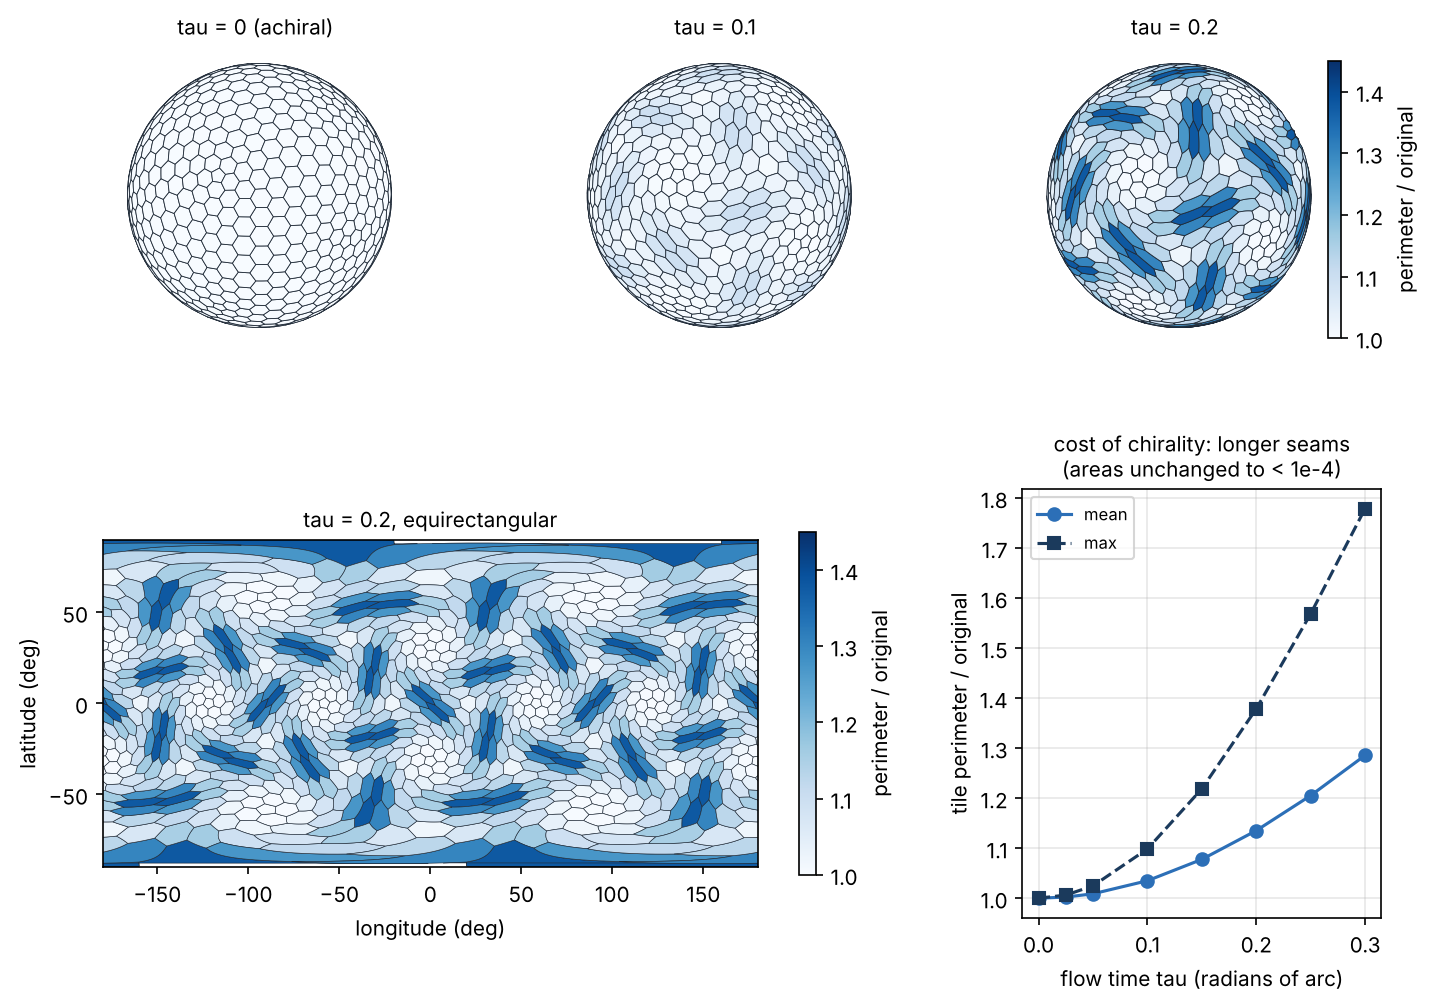
\includegraphics[width=\textwidth]{chiral_tilings}
\caption{The same flow construction applied to the hexagonal grid of the \texttt{hexasphere} repository (icosahedral grid, $n=8$, $812$ tiles). Top: the grid and its images for flow times $\tau=0$, $0.1$ and $0.2$; tiles are shaded by their perimeter relative to the undeformed tile. Bottom left: the $\tau=0.2$ tiling as an equirectangular map. Bottom right: mean and maximum tile perimeter against $\tau$. Every tile keeps its area (to within $10^{-4}$) and the tilings share their seams exactly; for $\tau>0$ all $60$ rotations of the icosahedron are kept and all $60$ improper symmetries are lost. Here $\tau$ is normalised to the largest distance, in radians of arc, that any point moves, so it is not the same scale as the flow time of the Trionda model.}\label{fig:chiralhex}
\end{figure}

\begin{figure}[htbp]
\centering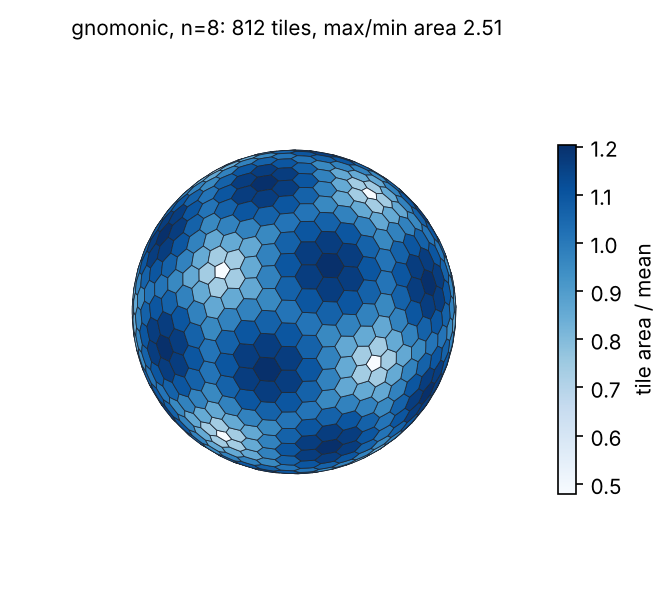
\includegraphics[width=\textwidth]{grid_3d_gnomonic}
\caption{The \texttt{hexasphere} grid with the gnomonic projection at resolution $n=8$: $812$ tiles, $12$ pentagons at the vertices of the icosahedron and $800$ hexagons. Tiles are shaded by area relative to the mean; the largest tile is $2.51$ times the smallest, and the pentagons are the smallest.}\label{fig:hexgrid}
\end{figure}


\bibliographystyle{plainnat}
\bibliography{refs}
\end{document}
